\RequirePackage{plautopatch}
% \documentclass[report,paper=a4, fontsize=12pt, line_length=16cm, number_of_lines=33]{jlreq}
% \usepackage[haranoaji,deluxe]{luatexja-preset}
% \usepackage{amsmath,amssymb}
% \usepackage{libertinus}

\documentclass[report,paper=a4, fontsize=12pt, line_length=16cm, number_of_lines=33,dvipdfmx]{jlreq}
\usepackage{jlreq-deluxe}
\usepackage{amsmath,amssymb}
\usepackage{stix2}
\renewcommand{\bfdefault}{bx}
% \usepackage{libertine}
% \usepackage{libertinust1math}
% \usepackage[T1]{fontenc}
% \usepackage{mlmodern}
% \usepackage[T1]{fontenc}
% \usepackage{tgtermes,tgheros,tgcursor}
% \renewcommand{\bfdefault}{bx}
% \usepackage[libertine]{newtxmath}

%% Fonts
%\usepackage{lmodern}
%\usepackage[T1]{fontenc}

\usepackage{tikz}
\usetikzlibrary{decorations,decorations.pathreplacing}
\usepackage{graphicx}
\graphicspath{{fig/}}

\usepackage{physics}
\usepackage{color}

\usepackage{tcolorbox}
\tcbuselibrary{breakable, skins, theorems}
%\usepackage{cleveref}

% font warningを出さないため
% \DeclareFontShape{JY2}{hgt}{b}{n}{<->ssub*hgt/bx/n}{}
% \DeclareFontShape{JY2}{hgt}{m}{it}{<->ssub*hgt/m/n}{}
% \DeclareFontShape{JT2}{hgt}{b}{n}{<->ssub*hgt/bx/n}{}
% \DeclareFontShape{JT2}{hgt}{m}{it}{<->ssub*hgt/m/n}{}
\newcommand{\qed}{■}
\newcommand{\kyou}[1]{{\sffamily \bfseries #1}}

\numberwithin{equation}{chapter}
%%%%%%%%%%%%%%%%%%%%%%%%%%%%%%%%%%%%%%%%%%%%%%%%%%%%%%%%%%%%%%%%%%%%%%
%                          often used macro
\newcommand{\del}{\partial}
\newcommand{\Cb}{\mathbb{C}}
\newcommand{\Zb}{\mathbb{Z}}
\newcommand{\CP}{\Cb \mathrm{P}}
%\newcommand{\strong}[1]{{\sffamily \gtfamily \bfseries #1}}
\newcommand{\Ztwo}{\mbox{$\mathbb{Z}_{2}$}}
\newcommand{\Hh}{\widehat{H}}
\newcommand{\Uh}{\widehat{U}}
\newcommand{\Vh}{\widehat{V}}
\newcommand{\Jh}{\widehat{J}}
\newcommand{\Qh}{\widehat{Q}}
\newcommand{\Oh}{\widehat{\mathcal{O}}}
\newcommand{\Gh}{\widehat{G}}
\newcommand{\ah}{\hat{a}}
\newcommand{\bh}{\hat{b}}
\newcommand{\Ocal}{\mathcal{O}}
\newcommand{\Ocalh}{\widehat{\mathcal{O}}}
\newcommand{\U}{\mbox{U}}
\newcommand{\ZIsing}{Z_{\mathrm{Ising}}}
\newcommand{\Zgauged}{Z_{\mathrm{Ising}/\Zb_2}}
\newcommand{\deltamod}[1]{\delta^{\mathrm{mod} \ 2}_{#1}}
\newcommand{\Kt}{\widetilde{K}}
\newcommand{\link}[1]{\expval{#1}}
\newcommand{\plaq}[1]{\expval{#1}}

\newcommand{\Ising}{\mbox{Ising}}
\newcommand{\gIsing}{\mbox{Ising$/\Zb_2$}}

\newcommand{\Tcal}{\mathcal{T}}

\newcommand{\underrem}[2]{
    {\color{red} \underbrace{\color{black} {#1}}_{\text{#2}}
    }
}

\newcommand{\overrem}[2]{
    {\color{red} \overbrace{\color{black} {#1}}^{\text{#2}}
    }
}


\colorlet{darkgreen}{green!70!black}
\colorlet{plaqblue}{blue!15}
\colorlet{linkblue}{blue!50}

\begin{document}

\begin{align}
    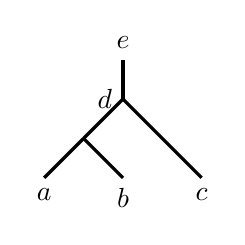
\begin{tikzpicture}[baseline=0]
        \draw[very thick](0,0)--(0.5,0.5) node [left]{$d$};
        \draw[very thick](0,0)--(-0.5,-0.5) node[below]{$a$};
        \draw[very thick](0,0)--(0.5,-0.5) node[below]{$b$};
        \draw[very thick](0.5,0.5)--(1.5,-0.5) node[below]{$c$};
        \draw[very thick](0.5,0.5)--(0.5,1) node[above]{$e$};
    \end{tikzpicture}
    \quad = \quad
    \sum_{f}
    (F_{abc}^e)_{df}
    \quad
    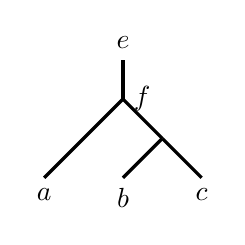
\begin{tikzpicture}[baseline=0]
        \draw[very thick](1,0)--(0.5,0.5) node [right]{$f$};
        \draw[very thick](0.5,0.5)--(-0.5,-0.5) node[below]{$a$};
        \draw[very thick](1,0)--(0.5,-0.5) node[below]{$b$};
        \draw[very thick](1,0)--(1.5,-0.5) node[below]{$c$};
        \draw[very thick](0.5,0.5)--(0.5,1) node[above]{$e$};
    \end{tikzpicture}            
\end{align}

\begin{align}
    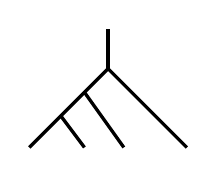
\begin{tikzpicture}[baseline=0]
        \draw[very thick](0.5,0.5)--(-0.5,-0.5);
        \draw[very thick](-0.1, -0.1)--(0.2,-0.5);
        \draw[very thick](0.2, 0.2)--(0.7,-0.5);
        \draw[very thick](0.5,0.5)--(1.5,-0.5);
        \draw[very thick](0.5,0.5)--(0.5,1);
    \end{tikzpicture}
    \quad = \quad
    F
    \quad
    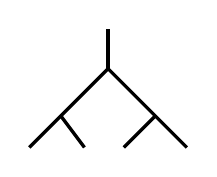
\begin{tikzpicture}[baseline=0]
        \draw[very thick](0.5,0.5)--(-0.5,-0.5);
        \draw[very thick](-0.1, -0.1)--(0.2,-0.5);
        \draw[very thick](1.1, -0.1)--(0.7,-0.5);
        \draw[very thick](0.5,0.5)--(1.5,-0.5);
        \draw[very thick](0.5,0.5)--(0.5,1);
    \end{tikzpicture}
    \quad = \quad
    FF\quad
    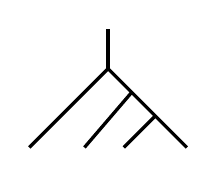
\begin{tikzpicture}[baseline=0]
        \draw[very thick](0.5,0.5)--(-0.5,-0.5);
        \draw[very thick](0.8, 0.2)--(0.2,-0.5);
        \draw[very thick](1.1, -0.1)--(0.7,-0.5);
        \draw[very thick](0.5,0.5)--(1.5,-0.5);
        \draw[very thick](0.5,0.5)--(0.5,1);
    \end{tikzpicture}
\end{align}

\begin{align}
    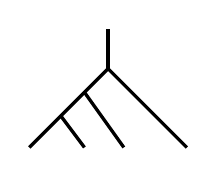
\begin{tikzpicture}[baseline=0]
        \draw[very thick](0.5,0.5)--(-0.5,-0.5);
        \draw[very thick](-0.1, -0.1)--(0.2,-0.5);
        \draw[very thick](0.2, 0.2)--(0.7,-0.5);
        \draw[very thick](0.5,0.5)--(1.5,-0.5);
        \draw[very thick](0.5,0.5)--(0.5,1);
    \end{tikzpicture}
    \quad = \quad
    F
    \quad
    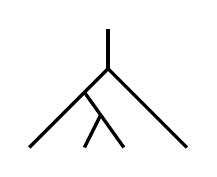
\begin{tikzpicture}[baseline=0]
        \draw[very thick](0.5,0.5)--(-0.5,-0.5);
        \draw[very thick](0.4, -0.1)--(0.2,-0.5);
        \draw[very thick](0.2, 0.2)--(0.7,-0.5);
        \draw[very thick](0.5,0.5)--(1.5,-0.5);
        \draw[very thick](0.5,0.5)--(0.5,1);
    \end{tikzpicture}
    \quad = \quad
    FF\quad
    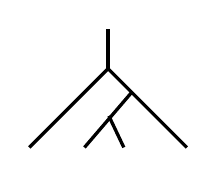
\begin{tikzpicture}[baseline=0]
        \draw[very thick](0.5,0.5)--(-0.5,-0.5);
        \draw[very thick](0.8, 0.2)--(0.2,-0.5);
        \draw[very thick](0.51, -0.1)--(0.7,-0.5);
        \draw[very thick](0.5,0.5)--(1.5,-0.5);
        \draw[very thick](0.5,0.5)--(0.5,1);
    \end{tikzpicture}
    \quad = \quad
    FFF\quad
    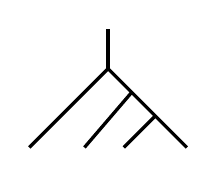
\begin{tikzpicture}[baseline=0]
        \draw[very thick](0.5,0.5)--(-0.5,-0.5);
        \draw[very thick](0.8, 0.2)--(0.2,-0.5);
        \draw[very thick](1.1, -0.1)--(0.7,-0.5);
        \draw[very thick](0.5,0.5)--(1.5,-0.5);
        \draw[very thick](0.5,0.5)--(0.5,1);
    \end{tikzpicture}
\end{align}

\begin{align}
    
\begin{tikzpicture}[baseline=0]
        \coordinate(A) at (-1,-1);
        \coordinate(B) at (1,-1);
        \coordinate(C) at (1,1);
        \coordinate(D) at (-1,1);
        \draw[darkgreen,thick](D)--(B);
        \draw[red,thick](A)--(-0.2,0.2);
        \draw[red,thick](C)--(0.2,-0.2);
    \end{tikzpicture} 
    \quad=\quad - \quad
    
\begin{tikzpicture}[baseline=0]
        \coordinate(A) at (-1,-1);
        \coordinate(B) at (1,-1);
        \coordinate(C) at (1,1);
        \coordinate(D) at (-1,1);
        \draw[darkgreen,thick](D)--(B);
        \draw[red,thick](A)--(0.2,-0.2);
        \draw[red,thick](C)--(-0.2,0.2);
    \end{tikzpicture} \quad ,
\end{align}

\begin{align}
    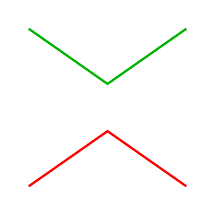
\begin{tikzpicture}[baseline=0]
        \coordinate(A) at (-1,-1);
        \coordinate(B) at (1,-1);
        \coordinate(C) at (1,1);
        \coordinate(D) at (-1,1);
        \draw[darkgreen,thick] (D)--(0,0.3)--(C);
        \draw[red,thick] (A)--(0,-0.3)--(B);
    \end{tikzpicture}
    \quad=
    \quad
    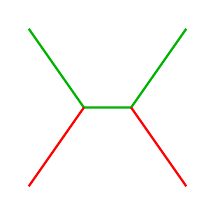
\begin{tikzpicture}[baseline=0]
        \coordinate(A) at (-1,-1);
        \coordinate(B) at (1,-1);
        \coordinate(C) at (1,1);
        \coordinate(D) at (-1,1);
        \draw[darkgreen,thick] (D)--(-0.3,0)--(0.3,0)--(C);
        \draw[red,thick] (A)--(-0.3,0);
        \draw[red,thick] (B)--(0.3,0);
    \end{tikzpicture}
    \quad
\end{align}

\begin{align}
    
\begin{tikzpicture}[baseline=0]
        \coordinate(A) at (-1,-1);
        \coordinate(B) at (1,-1);
        \coordinate(C) at (1,1);
        \coordinate(D) at (-1,1);
        \draw[darkgreen,thick] (D)--(0,0.3)--(C);
        \draw[darkgreen,thick] (A)--(0,-0.3)--(B);
    \end{tikzpicture}
    \quad=\quad \frac{1}{\sqrt{2}}\Bigg(
    \quad
    
\begin{tikzpicture}[baseline=0]
        \coordinate(A) at (-1,-1);
        \coordinate(B) at (1,-1);
        \coordinate(C) at (1,1);
        \coordinate(D) at (-1,1);
        \draw[darkgreen,thick] (D)--(-0.3,0)--(A);
        \draw[darkgreen,thick] (C)--(0.3,0)--(B);
    \end{tikzpicture}
    \quad
    +
    \quad
    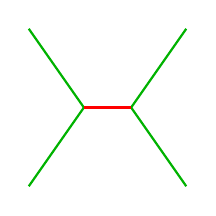
\begin{tikzpicture}[baseline=0]
        \coordinate(A) at (-1,-1);
        \coordinate(B) at (1,-1);
        \coordinate(C) at (1,1);
        \coordinate(D) at (-1,1);
        \draw[darkgreen,thick] (D)--(-0.3,0)--(A);
        \draw[darkgreen,thick] (C)--(0.3,0)--(B);
        \draw[red,thick] (0.3,0)--(-0.3,0);
    \end{tikzpicture}
    \quad
    \Bigg),
\end{align}

\begin{align}
    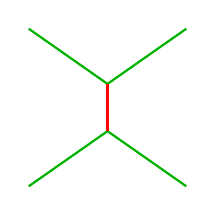
\begin{tikzpicture}[baseline=0]
        \coordinate(A) at (-1,-1);
        \coordinate(B) at (1,-1);
        \coordinate(C) at (1,1);
        \coordinate(D) at (-1,1);
        \draw[darkgreen,thick] (D)--(0,0.3)--(C);
        \draw[darkgreen,thick] (A)--(0,-0.3)--(B);
        \draw[red,thick] (0,0.3)--(0,-0.3);
    \end{tikzpicture}
    \quad=\quad \frac{1}{\sqrt{2}}\Bigg(
    \quad
    
\begin{tikzpicture}[baseline=0]
        \coordinate(A) at (-1,-1);
        \coordinate(B) at (1,-1);
        \coordinate(C) at (1,1);
        \coordinate(D) at (-1,1);
        \draw[darkgreen,thick] (D)--(-0.3,0)--(A);
        \draw[darkgreen,thick] (C)--(0.3,0)--(B);
    \end{tikzpicture}
    \quad
    -
    \quad
    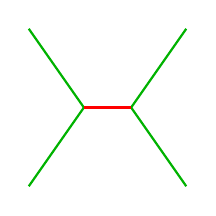
\begin{tikzpicture}[baseline=0]
        \coordinate(A) at (-1,-1);
        \coordinate(B) at (1,-1);
        \coordinate(C) at (1,1);
        \coordinate(D) at (-1,1);
        \draw[darkgreen,thick] (D)--(-0.3,0)--(A);
        \draw[darkgreen,thick] (C)--(0.3,0)--(B);
        \draw[red,thick] (0.3,0)--(-0.3,0);
    \end{tikzpicture}
    \quad
    \Bigg)
\end{align}


\begin{align}
    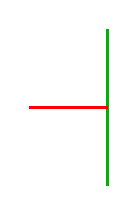
\begin{tikzpicture}[baseline=0]
        \draw[darkgreen,thick] (0,1)--(0,-1);
        \draw[red,thick] (-1,0)--(0,0);
    \end{tikzpicture}
    \quad
    =\quad
    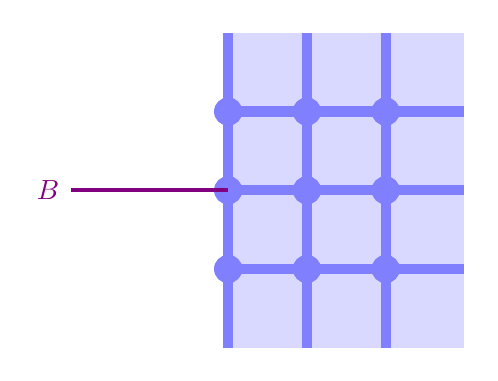
\begin{tikzpicture}[baseline=0cm]
        \foreach \x in {0,1,2}{
            \foreach \y in {-2,-1,...,1}{
            \fill[plaqblue](\x,\y) rectangle (\x+1,\y+1);
            }
        }
        \foreach \x in {0,1,2}{
            \foreach \y in {-1,0,1}{
                \fill[linkblue] (\x,\y) circle (1.8mm);
            }
        }
        \foreach \x in {0,1,2}{
            \foreach \y in {-1,0,1}{
                \draw[linkblue, line width = 1.3mm](\x,\y)--(\x + 1,\y);
            }
        }
        \foreach \x in {0,1,2}{
            \foreach \y in {-2,-1,...,1}{
                \draw[linkblue, line width = 1.3mm](\x,\y)--(\x,\y + 1);
            }
        }
        \draw[red!50!blue, ultra thick](0,0)--(-2,0) node[left]{$B$};
    \end{tikzpicture}        
\end{align}

\begin{align}
    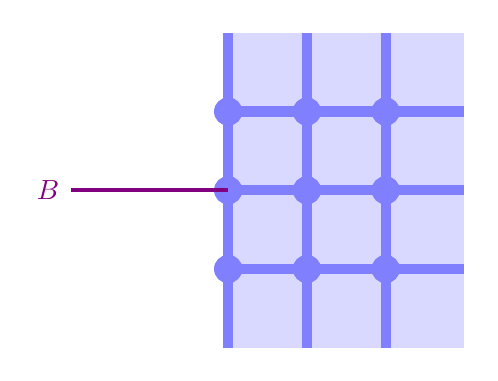
\begin{tikzpicture}[baseline=0cm]
        \foreach \x in {0,1,2}{
            \foreach \y in {-2,-1,...,1}{
            \fill[plaqblue](\x,\y) rectangle (\x+1,\y+1);
            }
        }
        \foreach \x in {0,1,2}{
            \foreach \y in {-1,0,1}{
                \fill[linkblue] (\x,\y) circle (1.8mm);
            }
        }
        \foreach \x in {0,1,2}{
            \foreach \y in {-1,0,1}{
                \draw[linkblue, line width = 1.3mm](\x,\y)--(\x + 1,\y);
            }
        }
        \foreach \x in {0,1,2}{
            \foreach \y in {-2,-1,...,1}{
                \draw[linkblue, line width = 1.3mm](\x,\y)--(\x,\y + 1);
            }
        }
        \draw[red!50!blue, ultra thick](0,0)--(-2,0) node[left]{$B$};
    \end{tikzpicture}
    \quad = \quad
    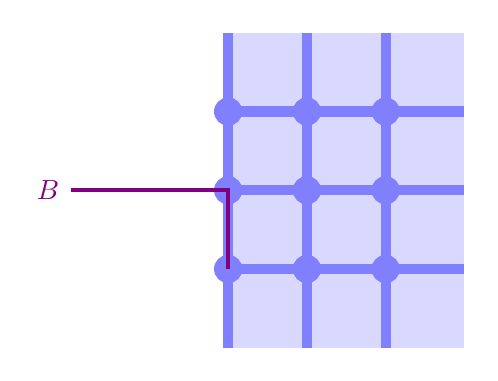
\begin{tikzpicture}[baseline=0cm]
        \foreach \x in {0,1,2}{
            \foreach \y in {-2,-1,...,1}{
            \fill[plaqblue](\x,\y) rectangle (\x+1,\y+1);
            }
        }
        \foreach \x in {0,1,2}{
            \foreach \y in {-1,0,1}{
                \fill[linkblue] (\x,\y) circle (1.8mm);
            }
        }
        \foreach \x in {0,1,2}{
            \foreach \y in {-1,0,1}{
                \draw[linkblue, line width = 1.3mm](\x,\y)--(\x + 1,\y);
            }
        }
        \foreach \x in {0,1,2}{
            \foreach \y in {-2,-1,...,1}{
                \draw[linkblue, line width = 1.3mm](\x,\y)--(\x,\y + 1);
            }
        }
        \draw[red!50!blue, ultra thick](0,-1)--(0,0)--(-2,0) node[left]{$B$};
    \end{tikzpicture}    
    \quad \notag \\= \quad
    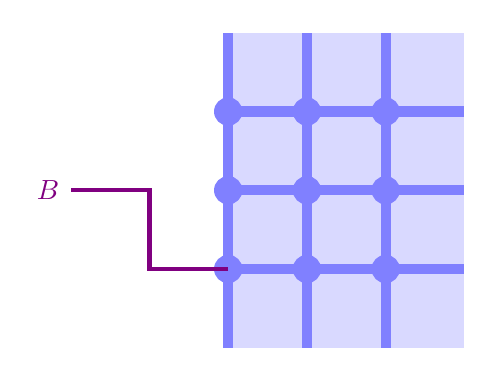
\begin{tikzpicture}[baseline=0cm]
        \foreach \x in {0,1,2}{
            \foreach \y in {-2,-1,...,1}{
            \fill[plaqblue](\x,\y) rectangle (\x+1,\y+1);
            }
        }
        \foreach \x in {0,1,2}{
            \foreach \y in {-1,0,1}{
                \fill[linkblue] (\x,\y) circle (1.8mm);
            }
        }
        \foreach \x in {0,1,2}{
            \foreach \y in {-1,0,1}{
                \draw[linkblue, line width = 1.3mm](\x,\y)--(\x + 1,\y);
            }
        }
        \foreach \x in {0,1,2}{
            \foreach \y in {-2,-1,...,1}{
                \draw[linkblue, line width = 1.3mm](\x,\y)--(\x,\y + 1);
            }
        }
        \draw[red!50!blue, ultra thick](0,-1)--(-1,-1)--(-1,0)--(-2,0) node[left]{$B$};
    \end{tikzpicture}    
\end{align}


\begin{align}
    \begin{tikzpicture}[baseline=0]
        \draw[darkgreen,thick] (0,1)--(0,-1);
        \draw[red,thick] (1,0)--(0,0);
    \end{tikzpicture}
    \quad
    =\quad
    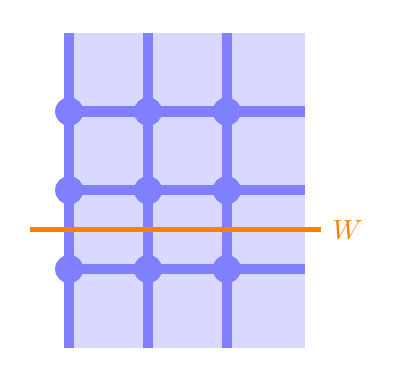
\begin{tikzpicture}[baseline=0cm]
        \foreach \x in {0,1,2}{
            \foreach \y in {-2,-1,...,1}{
            \fill[plaqblue](\x,\y) rectangle (\x+1,\y+1);
            }
        }
        \foreach \x in {0,1,2}{
            \foreach \y in {-1,0,1}{
                \fill[linkblue] (\x,\y) circle (1.8mm);
            }
        }
        \foreach \x in {0,1,2}{
            \foreach \y in {-1,0,1}{
                \draw[linkblue, line width = 1.3mm](\x,\y)--(\x + 1,\y);
            }
        }
        \foreach \x in {0,1,2}{
            \foreach \y in {-2,-1,...,1}{
                \draw[linkblue, line width = 1.3mm](\x,\y)--(\x,\y + 1);
            }
        }
        \draw[red!50!yellow, ultra thick](-0.5,-0.5)--(3.2,-0.5) node[right]{$W$};
    \end{tikzpicture}        
\end{align}

\begin{align}
    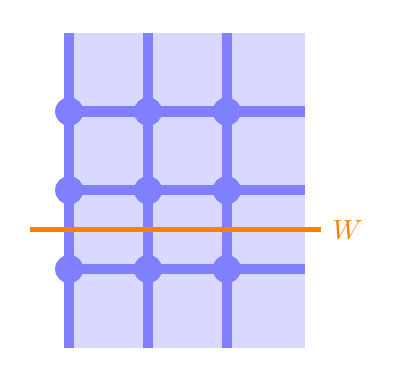
\begin{tikzpicture}[baseline=0cm]
        \foreach \x in {0,1,2}{
            \foreach \y in {-2,-1,...,1}{
            \fill[plaqblue](\x,\y) rectangle (\x+1,\y+1);
            }
        }
        \foreach \x in {0,1,2}{
            \foreach \y in {-1,0,1}{
                \fill[linkblue] (\x,\y) circle (1.8mm);
            }
        }
        \foreach \x in {0,1,2}{
            \foreach \y in {-1,0,1}{
                \draw[linkblue, line width = 1.3mm](\x,\y)--(\x + 1,\y);
            }
        }
        \foreach \x in {0,1,2}{
            \foreach \y in {-2,-1,...,1}{
                \draw[linkblue, line width = 1.3mm](\x,\y)--(\x,\y + 1);
            }
        }
        \draw[red!50!yellow, ultra thick](-0.5,-0.5)--(3.2,-0.5) node[right]{$W$};
    \end{tikzpicture}
    \quad
    =\quad
    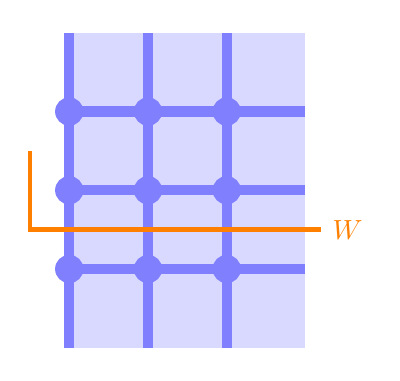
\begin{tikzpicture}[baseline=0cm]
        \foreach \x in {0,1,2}{
            \foreach \y in {-2,-1,...,1}{
            \fill[plaqblue](\x,\y) rectangle (\x+1,\y+1);
            }
        }
        \foreach \x in {0,1,2}{
            \foreach \y in {-1,0,1}{
                \fill[linkblue] (\x,\y) circle (1.8mm);
            }
        }
        \foreach \x in {0,1,2}{
            \foreach \y in {-1,0,1}{
                \draw[linkblue, line width = 1.3mm](\x,\y)--(\x + 1,\y);
            }
        }
        \foreach \x in {0,1,2}{
            \foreach \y in {-2,-1,...,1}{
                \draw[linkblue, line width = 1.3mm](\x,\y)--(\x,\y + 1);
            }
        }
        \draw[red!50!yellow, ultra thick](-0.5, 0.5)--(-0.5,-0.5)--(3.2,-0.5) node[right]{$W$};
    \end{tikzpicture}
    \quad
    =\quad
    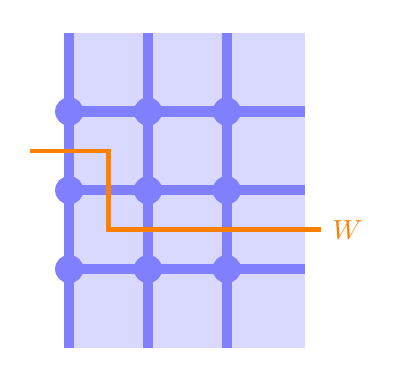
\begin{tikzpicture}[baseline=0cm]
        \foreach \x in {0,1,2}{
            \foreach \y in {-2,-1,...,1}{
            \fill[plaqblue](\x,\y) rectangle (\x+1,\y+1);
            }
        }
        \foreach \x in {0,1,2}{
            \foreach \y in {-1,0,1}{
                \fill[linkblue] (\x,\y) circle (1.8mm);
            }
        }
        \foreach \x in {0,1,2}{
            \foreach \y in {-1,0,1}{
                \draw[linkblue, line width = 1.3mm](\x,\y)--(\x + 1,\y);
            }
        }
        \foreach \x in {0,1,2}{
            \foreach \y in {-2,-1,...,1}{
                \draw[linkblue, line width = 1.3mm](\x,\y)--(\x,\y + 1);
            }
        }
        \draw[red!50!yellow, ultra thick](-0.5, 0.5)--(0.5, 0.5)--(0.5,-0.5)--(3.2,-0.5) node[right]{$W$};
    \end{tikzpicture}
\end{align}

\begin{align}
    \begin{tikzpicture}[baseline=0]
        \draw[darkgreen,thick] (0,1)--(0,-1);
        \draw[red,thick] (-1,0)--(0,0);
        \draw[red,thick] (1,-0.3)--(0,-0.3);
    \end{tikzpicture}
    \quad
    &=\quad
    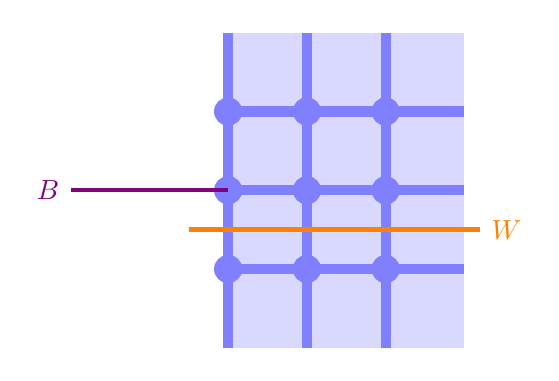
\begin{tikzpicture}[baseline=0cm]
        \foreach \x in {0,1,2}{
            \foreach \y in {-2,-1,...,1}{
            \fill[plaqblue](\x,\y) rectangle (\x+1,\y+1);
            }
        }
        \foreach \x in {0,1,2}{
            \foreach \y in {-1,0,1}{
                \fill[linkblue] (\x,\y) circle (1.8mm);
            }
        }
        \foreach \x in {0,1,2}{
            \foreach \y in {-1,0,1}{
                \draw[linkblue, line width = 1.3mm](\x,\y)--(\x + 1,\y);
            }
        }
        \foreach \x in {0,1,2}{
            \foreach \y in {-2,-1,...,1}{
                \draw[linkblue, line width = 1.3mm](\x,\y)--(\x,\y + 1);
            }
        }
        \draw[red!50!yellow, ultra thick](-0.5,-0.5)--(3.2,-0.5) node[right]{$W$};
        \draw[red!50!blue, ultra thick](0,0)--(-2,0) node[left]{$B$};
    \end{tikzpicture}
    \notag\\
    &=\quad - \quad
    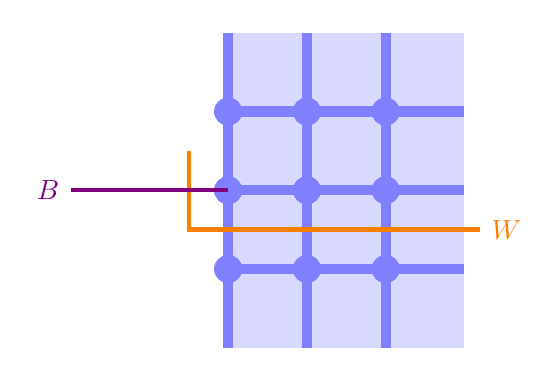
\begin{tikzpicture}[baseline=0cm]
        \foreach \x in {0,1,2}{
            \foreach \y in {-2,-1,...,1}{
            \fill[plaqblue](\x,\y) rectangle (\x+1,\y+1);
            }
        }
        \foreach \x in {0,1,2}{
            \foreach \y in {-1,0,1}{
                \fill[linkblue] (\x,\y) circle (1.8mm);
            }
        }
        \foreach \x in {0,1,2}{
            \foreach \y in {-1,0,1}{
                \draw[linkblue, line width = 1.3mm](\x,\y)--(\x + 1,\y);
            }
        }
        \foreach \x in {0,1,2}{
            \foreach \y in {-2,-1,...,1}{
                \draw[linkblue, line width = 1.3mm](\x,\y)--(\x,\y + 1);
            }
        }
        \draw[red!50!yellow, ultra thick](-0.5, 0.5)--(-0.5,-0.5)--(3.2,-0.5) node[right]{$W$};
        \draw[red!50!blue, ultra thick](0,0)--(-2,0) node[left]{$B$};
    \end{tikzpicture}
    \notag\\
    &=\quad - \quad
    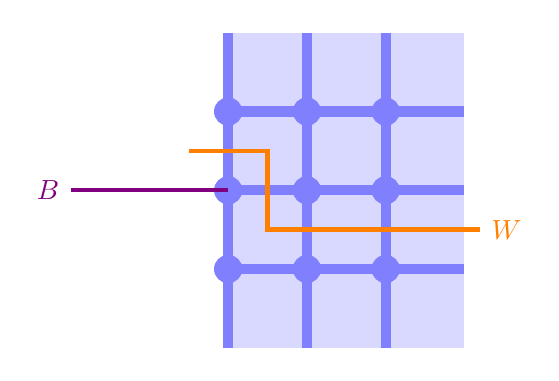
\begin{tikzpicture}[baseline=0cm]
        \foreach \x in {0,1,2}{
            \foreach \y in {-2,-1,...,1}{
            \fill[plaqblue](\x,\y) rectangle (\x+1,\y+1);
            }
        }
        \foreach \x in {0,1,2}{
            \foreach \y in {-1,0,1}{
                \fill[linkblue] (\x,\y) circle (1.8mm);
            }
        }
        \foreach \x in {0,1,2}{
            \foreach \y in {-1,0,1}{
                \draw[linkblue, line width = 1.3mm](\x,\y)--(\x + 1,\y);
            }
        }
        \foreach \x in {0,1,2}{
            \foreach \y in {-2,-1,...,1}{
                \draw[linkblue, line width = 1.3mm](\x,\y)--(\x,\y + 1);
            }
        }
        \draw[red!50!yellow, ultra thick](-0.5, 0.5)--(0.5, 0.5)--(0.5,-0.5)--(3.2,-0.5) node[right]{$W$};
        \draw[red!50!blue, ultra thick](0,0)--(-2,0) node[left]{$B$};
    \end{tikzpicture}
    \notag \\
    &=\quad -\quad
    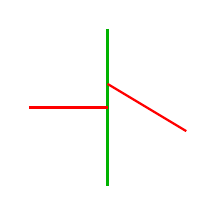
\begin{tikzpicture}[baseline=0]
        \draw[darkgreen,thick] (0,1)--(0,-1);
        \draw[red,thick] (-1,0)--(0,0);
        \draw[red,thick] (1,-0.3)--(0,0.3);
    \end{tikzpicture}
\end{align}


\begin{align}
    
\begin{tikzpicture}[baseline=0]
        \coordinate(A) at (-1,-1);
        \coordinate(B) at (1,-1);
        \coordinate(C) at (1,1);
        \coordinate(D) at (-1,1);
        \draw[darkgreen,thick] (D)--(0,0.3)--(C);
        \draw[darkgreen,thick] (A)--(0,-0.3)--(B);
    \end{tikzpicture}
    \quad=\quad 
    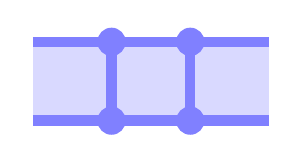
\begin{tikzpicture}[baseline=0.5cm]
        \foreach \x in {0,1,2}{
            \foreach \y in {-2,-1,...,1}{
            \fill[plaqblue](\x,0) rectangle (\x+1,1);
            }
        }
        \foreach \x in {1,2}{
            \foreach \y in {0,1}{
                \fill[linkblue] (\x,\y) circle (1.8mm);
            }
        }
        \foreach \x/\y in {0/0,1/0,2/0,0/1,1/1,2/1}{
                \draw[linkblue, line width = 1.3mm](\x,\y)--(\x + 1,\y);
        }
        \foreach \x in {1,2}{
            \draw[linkblue, line width = 1.3mm](\x,0)--(\x, 1);
        }
    \end{tikzpicture}
    \quad=\quad 
    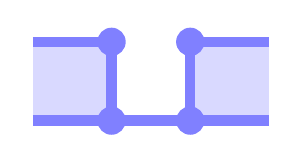
\begin{tikzpicture}[baseline=0.5cm]
        \foreach \x in {0,2}{
            \foreach \y in {-2,-1,...,1}{
            \fill[plaqblue](\x,0) rectangle (\x+1,1);
            }
        }
        \foreach \x in {1,2}{
            \foreach \y in {0,1}{
                \fill[linkblue] (\x,\y) circle (1.8mm);
            }
        }
        \foreach \x/\y in {0/0,1/0,2/0,0/1,2/1}{
                \draw[linkblue, line width = 1.3mm](\x,\y)--(\x + 1,\y);
        }
        \foreach \x in {1,2}{
            \draw[linkblue, line width = 1.3mm](\x,0)--(\x, 1);
        }
    \end{tikzpicture}   
\end{align}

\begin{align}
    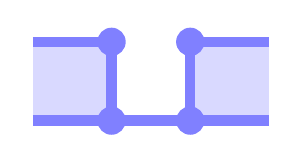
\begin{tikzpicture}[baseline=0.5cm]
        \foreach \x in {0,2}{
            \foreach \y in {-2,-1,...,1}{
            \fill[plaqblue](\x,0) rectangle (\x+1,1);
            }
        }
        \foreach \x in {1,2}{
            \foreach \y in {0,1}{
                \fill[linkblue] (\x,\y) circle (1.8mm);
            }
        }
        \foreach \x/\y in {0/0,1/0,2/0,0/1,2/1}{
                \draw[linkblue, line width = 1.3mm](\x,\y)--(\x + 1,\y);
        }
        \foreach \x in {1,2}{
            \draw[linkblue, line width = 1.3mm](\x,0)--(\x, 1);
        }
    \end{tikzpicture}
    \quad = \frac{1}{\sqrt{2}}\left(
        
\begin{tikzpicture}[baseline=0.5cm]
            \foreach \x in {0,2}{
                \foreach \y in {-2,-1,...,1}{
                \fill[plaqblue](\x,0) rectangle (\x+1,1);
                }
            }
            \foreach \x in {1,2}{
                \foreach \y in {0,1}{
                    \fill[linkblue] (\x,\y) circle (1.8mm);
                }
            }
            \foreach \x/\y in {0/0,2/0,0/1,2/1}{
                    \draw[linkblue, line width = 1.3mm](\x,\y)--(\x + 1,\y);
            }
            \foreach \x in {1,2}{
                \draw[linkblue, line width = 1.3mm](\x,0)--(\x, 1);
            }
        \end{tikzpicture}
        \quad + \quad
        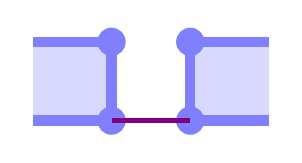
\begin{tikzpicture}[baseline=0.5cm]
            \foreach \x in {0,2}{
                \foreach \y in {-2,-1,...,1}{
                \fill[plaqblue](\x,0) rectangle (\x+1,1);
                }
            }
            \foreach \x in {1,2}{
                \foreach \y in {0,1}{
                    \fill[linkblue] (\x,\y) circle (1.8mm);
                }
            }
            \foreach \x/\y in {0/0,2/0,0/1,2/1}{
                    \draw[linkblue, line width = 1.3mm](\x,\y)--(\x + 1,\y);
            }
            \foreach \x in {1,2}{
                \draw[linkblue, line width = 1.3mm](\x,0)--(\x, 1);
            }
            \draw[red!50!blue, ultra thick](1,0)--(2,0);
        \end{tikzpicture}        
    \right)
\end{align}
\end{document}  